\subsection{System Model}
\label{formulation}

Consider a hexrotor, which is an autonomous flying robot with six rotors, shown in Fig.~\ref{fig:nanohex}.
The state $\stPt$ of the hexrotor is made of its 3D position and 3D velocity.
The input $\inpPt$ to the robot consists of the desired pitch and roll angles, and the desired thrust.
The hexrotor's mission is to fly a pre-defined pattern given by $\stPt_{ref}$, where $\stPt_{ref}(t)$ gives the desired position at each time $t$.
The dynamics of the hexrotor, relating the time-evolution of its state to the current state and input, can be linearized and approximated by the following Linear Time-Invariant (LTI) ODE:
\begin{equation}
\dot{x}(t) = A_{c}x(t)+B_{c}u(t)+w_{c}(t)  \label{eq:plant-cont-model}
\end{equation}
where $x\in \Re^{n}$ is the state constrained to lie in a set $\stSet \subset \Re^n$,
$\inpPt\in\Re^{m}$ is the control input constrained to lie in a set $\inpSet \subset \Re^m$,
and $w_{c}\in\Re^{n}$ is the bounded process noise assumed to lie in a set $\Wc_c \subset \Re^n$.
$A_c \in \Re^{n\times n}$ and $B_c \in \Re^{m\times n}$ are matrices.
LTIs model a wide range of systems, and our results apply to arbitrary LTIs of the form given in \eqref{eq:plant-cont-model} with compact and convex constraint sets $\stSet,\inpSet$ and $\Wc_c$.
The sets $\stSet$ and $\inpSet$ are part of the problem statement and are either chosen by the designer or determined by physical constraints of the physical plant and the actuators.
For the hexrotor, $\stSet$ captures limits on the state such that the LTI dynamics provide a good approximation of the true nonlinear dynamics.
The set $\inpSet$ restricts the inputs to values that can be supported by the rotors.

\subsection{Time-Triggered Sensing and Actuation}
For flight the hexrotor needs to determine its current position and speed, i.e., it needs to produce an \emph{estimate} of its current state $\stPt$.
It does so by taking a video during flight through a downward facing camera, detecting and tracking features across frames, and deducing its own position relative to these features.
The camera captures a new frame every $T > 0$ seconds, thus resulting in periodic measurements at instants $t_{s,k}=kT$,
where $k\in\Ne$.
\begin{figure}[t]
\centering
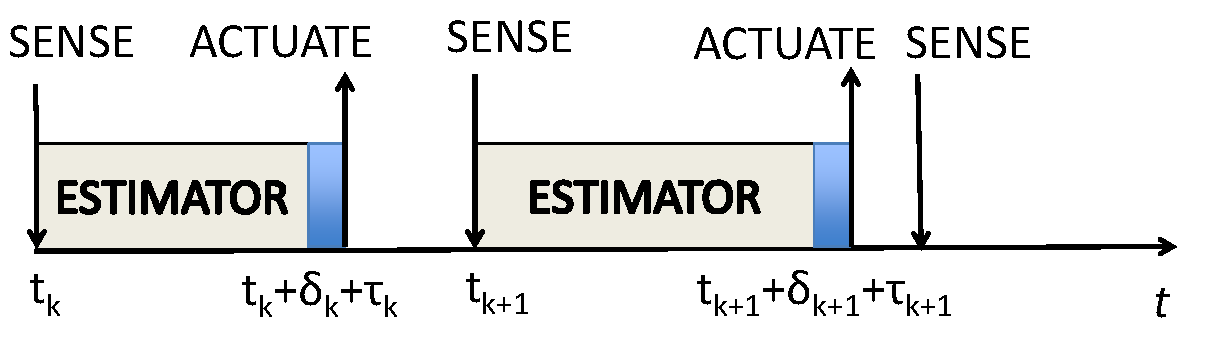
\includegraphics[width=0.7\linewidth]{figures/senseActuate}
\caption{Time-triggered sensing and actuation.}
\label{fig:senseActuate}
\end{figure}

The sampled measurement is fed to the estimator that computes the state
estimate $\hat{x}_{k}\defeq\hat{x}(t_{s,k})$ with the desired
accuracy $\sAccu_k$ \emph{determined by the controller in the previous time step}.
The controller then uses this state estimate
to compute the control input $u_{k}$ as well as decide on the
state estimate's delay and accuracy contract $(\sDelay_{k+1},\sAccu_{k+1})$ for the next step.
This control is applied to the physical system according to \eqref{eq:plant-cont-model} at instant $t_{a,k} = t_{s,k}+\sDelay_k + \tau_k$, where $\tau_k$ is the time it takes to compute the input. 
See Fig.~\ref{fig:senseActuate}.

In our setting, the controller has access to the delay-error curve $\Delta$ of the estimator, and makes contract selections \emph{from that curve}.
This curve is obtained offline as explained in Section \ref{sec:codesign}, and exemplified in Section \ref{delayErrorCurve}.
We remark that in each step $k\geq0$, the estimation accuracy $\sAccu_k$
and hence the delay $\sDelay_k$ are already decided in the previous
step and known to the controller.
In the first step $k=0$, the
initial accuracy $\sAccu_0$, the initial delay $\sDelay_0$, and
the initial control input $u_{-1}$ are chosen by the designer.

\subsection{Control Performance}
The goal of the controller is twofold: it needs to ensure that the reference pattern is adhered to as closely as possible, and that the energy consumed to fly this pattern is minimized.
Thus we may define two (stage) cost functions: first, $\ell(\stPt, \inpPt) = (\stPt - \stPt_{ref})^TQ(\stPt - \stPt_{ref}) + \inpPt^T R \inpPt$ defines a weighted sum of the tracking error (first summand) and the input power (second summand).
Here, $Q$ and $R$ are positive semidefinite matrices.
Second, $\pi(\sDelay)$ captures the average power consumed to perform an estimation of duration $\sDelay$.
This power information is collected offline during the estimator profiling phase.
The paper's formulation holds for much more general stage cost functions.
These stage cost functions are chosen by the designer to achieve a desired control performance.

The total cost function that the controller minimizes is then
\(
J=\sum_{k=0}^{M}\left(\ell(\stPt_k,\inpPt_k)+ \alpha \pi(\sDelay_k)\right)
\),
where $M \geq 0$ is the duration of the system's operation.

\subsection{Discretized Dynamics}
Because of time-triggered sensing and actuation, from time $t_{s,k}$ to $t_{a,k}$, the  previous control input $u_{k-1}$
is still used.
Then at $t_{a,k}$ the new control input $u_{k}$
is computed and applied by the controller (see Fig.~\ref{fig:senseActuate}).
The discretized dynamics are given by
\begin{equation}
\label{eq:disc-dynamics}
x_{k+1}=Ax_{k}+B_{1}(\sDelay_k)u_{k-1}+B_{2}(\sDelay_k)u_{k}+w_{k}, k\geq0
\end{equation}
in which
\begin{eqnarray*}
&A=\eu^{A_{c}T}, \quad
w_{k}%=\int_{t_{s,k}}^{t_{s,k+1}}\eu^{A_{c}(t_{s,k+1}-t)}w_{c}(t)\diff t \nonumber \\
=\int_{0}^{T}\eu^{A_{c}(T-t)}w_{c}(t_{s,k}+t) dt
\\
&B_{1}(\sDelay)%=\int_{t_{s,k}}^{t_{a,k}}\eu^{A_{c}(t_{s,k+1}-t)}B_{c}\diff t
\!=\!\int_{0}^{\sDelay}\eu^{A_{c}(T-t)}B_{c} dt,\,
B_{2}(\sDelay)%=\int_{t_{a,k}}^{t_{s,k+1}}\eu^{A_{c}(t_{s,k+1}-t)}B_{c}\diff t
\!=\!\int_{\sDelay}^{T}\eu^{A_{c}(T-t)}B_{c} dt \text.
\end{eqnarray*}
Here $w_{k}$ is the accumulated process noise during the interval, and is constrained to lie in a compact convex set $\Wc$ because $w_c(t)$ lies in the compact convex set $\Wc_c$ and $T$ is finite.
Note that both the current control $u_{k}$ and the previous
control $u_{k-1}$ appear in \eqref{eq:disc-dynamics}.
Furthermore, the input matrices $B_{1}(\sDelay_k)$ and $B_{2}(\sDelay_k)$
depend on the delay $\sDelay_k$.
The estimation accuracy $\sAccu_k$ affects the state estimate
$\hat{\stPt}_{k}$ %which is
used by the controller to compute $u_{k}$;
therefore $\sAccu_k$ indirectly affects the dynamics via the control
input.







